\chapter{Realisierung}\label{ch:realisierung_der_anwendung}
In den nachfolgenden Abschnitten werden alle für die Anwendung wichtigen Aspekte und deren Umsetzung erläutert. 

\section{Einbindung der Mustererkennung}\label{einbindung_mustererkennung}
In Abschnitt \ref{mustererkennung_vuforia} haben wir uns bereits mit der internen Funktionsweise des Augmented Reality Frameworks \textquote{Vuforia} beschäftigt. 
Damit wir dessen vollen Umfang in der Unity-Projektumgebung nutzen können, mussten wir das entsprechende Vuforia Software Development Kit einbinden.
Es beinhaltet im wesentlichen alle Grundbausteine für die Entwicklung einer Augmented Reality App und stellt diese in Form von Unity GameObjects bereit. 
Dadurch sind sie genau wie herkömmliche GameObjects nutzbar.
Sie können ganz einfach in ein bestehendes Unity-Projekt integriert werden und dieses erweitern.

Beispiele für ein paar der Bausteine wären zum einen die AR Camera. 
Sie beinhaltet Logik um die Hauptkamera des ausführenden Gerätes anzusteuern. Die Szene in der die Kamera platziert wurde, wird nun in das Kamerabild der realen Welt projiziert.
Dieser Baustein ist essentiell für die Erstellung einer Augmented Reality App. 

Auf einen Weiteren essentiellen Baustein aus der Vuforia SDK wird in den nachfolgenden Unterabschnitten \ref{image_targets} und \ref{integration_image_targets} eingegangen. 

\subsection{Image Targets}\label{image_targets}
Da wir uns in der Anwendung für die markerbasierte Variante der Augmented Reality entschieden haben, benötigen wir hierzu die passenden Marker. 
Wie bereits in Abschnitt \ref{mustererkennung_vuforia} beschrieben, bietet Vuforia hier die Möglichkeit eigene Image Targets zu verwenden. 
Da diese innerhalb der Anwendung möglichst gut erkannt werden sollen, müssen bei der Wahl der Bilder einige Qualitätskriterien beachtet werden.

Eines dieser Kriterien sind die Ecken und Kanten im Bild, welche durch die Featureextraktion beim hochladen des Bildes berücksichtigt werden. 
Jede scharfe Ecke und Kante wird als Feature abgespeichert und dient später, bei der Bilderkennung innerhalb der Anwendung als Vergleichsmerkmal. 
Je mehr dieser markanten Punkte im Bild vorhanden sind, desto leichter fällt es der Vuforia Engine das Image Target im Kamerabild der AR-Anwendung zu identifizieren.

Um sicherzugehen, dass aus dem gewählten Image Target viele Features extrahiert werden können, muss das Bild hohe lokale Kontraste besitzen. Das heißt es muss genügend Stellen geben, an denen sehr helle Pixel neben sehr dunklen liegen. 
Hiermit ergeben sich ausgeprägte Farbunterschiede und somit schärfere Ecken und Kanten, welche als potentielle Features in Frage kommen.

\begin{figure} [h]
\centering
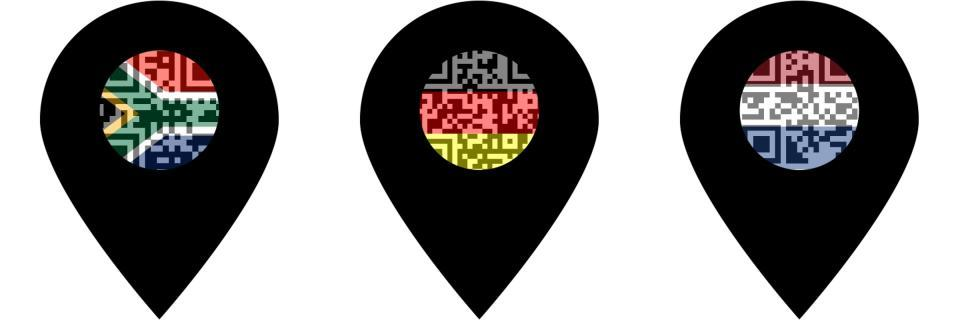
\includegraphics[width=12cm]{Image_Targets.jpg}
\caption{Beispiele der verwendeten Image Targets}
\label{fig:image_targets}
\end{figure}

In der Abbildung \ref{fig:image_targets} sind die finalen Image Targets der beschriebenen Anwendung zu sehen.
Die Grundform der Targets stellt die heutzutage sehr häufig genutzte Form des Standortsymbols dar.
Wir wählten die Form aufgrund ihrer Intuitivität im Anbetracht der gesamten Thematik der Anwendung.
Diese werden in der Praxis auf einem Globus platziert und jedes der Targets repräsentiert ein Land.
Um die Verbindung zu dem jeweiligem Land erkenntlich zu machen, bauten wir die Flagge des Landes mit in das Standortsymbol ein. 
Somit ist jedes Image Target einzigartig und lässt sich von den anderen unterscheiden. 
Der Nutzer der Anwendung kann jetzt erkennen, welches Image Target zu welchem Land gehört und gleichzeitig kann er sich die Flaggen der Länder einprägen. 

Nun sind zwar alle Targets einzigartig und können in manchen Fällen sehr gut unterschieden werden, jedoch ist das noch nicht genug um bei der Targeterkennung befriedigende Ergebnisse zu erhalten. 
Bei der Merkmalsextraktion werden die Bilder in Graustufen umgewandelt und verlieren somit jegliche Farbinformationen. Dies kann beispielsweise bei den Flaggen von Deutschland und den Niederlanden zu Schwierigkeiten in der Unterscheidung führen, da sie aus den exakt gleichen Formen bestehen. 
Die Ecken- und Kantenmerkmale wären damit exakt die selben. 
Um dieses Problem zu lösen hinterlegten wir jede Flagge mit einem individuellem QR-Code. Dieser ist leicht transparent, bringt aber dennoch mehr Kontrast in das Bild. 
Somit können selbst aus den einfach geformten Flaggen genügend eindeutige Merkmale erzeugt werden.

Diese Art der Image Targets resultiert in der Vuforia Engine in einer Fünf-Sterne Erkennungsrate.

\subsection{Integration der Image Targets}\label{integration_image_targets}
Nachdem nun alle fertigen Image Targets in die Vuforia-Weboberfläche geladen wurden, müssen diese ihren Weg in die Anwendungsumgebung finden.
Hierzu wird aus der Weboberfläche eine Datenbank erzeugt, die alle Targets enthält. 
Anschließend wird diese als \textquote{.unitypackage}-Datei heruntergeladen und kann ganz einfach in das bestehende Unityprojekt importiert werden.

Um nun die einzelnen Image Targets innerhalb der Anwendung nutzbar zu machen, erstellten wir zunächst eine dedizierte Szene. 
In dieser Szene befindet sich zuerst einmal die AR Camera, welche in Abschnitt \ref{einbindung_mustererkennung} beschrieben ist. 
Des Weiteren benötigen wir für jedes vorhandene Land das passende Target.
Ein Image Target wird in Form eines GameObjects in die Szene geladen.
Es ist ein spezieller Typ von GameObjects, welcher von der Vuforia-SDK mitgebracht wird.
Dieser Typ enthält bereits vordefinierte Logik in Form von Komponenten. 
Zum Beispiel die Scriptkomponente \textquote{Image Target Behaviour}, welche die Kommunikation mit der Image Target Datenbank regelt. 
Sie beitet die Möglichkeit zwischen allen importierten Datenbanken und den darin enthaltenen Image Targets zu wählen.
Wählt man jetzt beim ersten GameObject das Target des Landes Indien, so erscheint an der Stelle des vorher leeren Objekts, das erstellte Image Target für genau dieses Land.
Dies müssen wir nun für alle restlichen Länder wiederholen, damit alle in der Szene enthalten sind.

Wenn nun die fertige Szene gestartet wird, öffnet sich zunächst die Kamera des ausführenden Geräts.
Im Hintergrund wird das Kamerabild ständig untersucht und geprüft, ob sich eines der in der Szene liegenden Image Targets im Sichtfeld befindet. Was daraufhin passiert wird in Abschnitt \ref{einbindung_3D_objekte} beschrieben.

\section{Verwendung von 3D Objekten}\label{verwendung_3d_objekte}
Die in der Anwendung verwendeten 3D Objekte liegen im \textquote{object}-Format vor, welches durch die Dateiendung \textquote{.obj} gekennzeichnet ist. 
Dem Dateiformat liegt das polygonale Modell zugrunde, das 3D Objekte als Zusammensetzung von Polygonen, die wiederum aus durch Kanten verbundenen Koordinaten bestehen, definiert. 
Die geläufigsten so entstehenden Polygonnetze sind Dreiecksnetze und Vierecksnetze.

In einer  \textquote{.obj}-Datei sind somit die Koordinaten von Punkten im dreidimensionalen Raum definiert, welche über Kantendefinitionen zu Flächen verbunden werden. 
Um 3D Objekte realistisch erscheinen zu lassen, findet der Prozess des sogenannten \textquote{Texture Mappings} statt, in welchem eine Textur im Bildformat über ein 3D Objekt gelegt wird. 
Auf Codebasis wird dies realisiert, indem in der \textquote{.obj}-Datei zweidimensionale Texturkoordinaten für eine vorhandene Textur definiert und bestimmten Punktkoordinaten des Objekts zugewiesen werden.

Primitive 3D Objekte, die aus wenigen Polygonen bestehen, können somit leicht selbst erstellt werden, während die Erstellung von komplexeren Objekten und zugehörigen Texturen mehr Zeitaufwand erfordert. 
Da dieser Zeitaufwand nicht in den zeitlichen Rahmen dieses IT Projektes gepasst hat, haben wir uns dafür entschieden, kostenlose 3D Objekte mit zugehörigen Texturen von verschiedenen Anbietern aus dem Internet zu verwenden, welche im folgenden aufgelistet sind.

\begin{itemize}
\item https://www.turbosquid.com/
\item https://www.cgtrader.com/
\item https://free3d.com/
\end{itemize}

Wie bereits in Abschnitt \ref{projektziel} erwähnt, sollen die Länder, die in der App enthalten sind durch passende 3D Objekte repräsentiert werden, welche auf das erkannten Image Target eines Landes gerendert werden. 
Die folgende Auflistung zeigt die gewählten 3D Objekte für ihre zugehörigen Länder, gegliedert in Kontinente. Diese sind bildlich auch im Anhang dargestellt.

\textbf{3D Objekte für Afrika:}
\begin{itemize}
\item Kongo: Affe
\item Südafrika: Elefant
\item Ägypten: Pyramide
\end{itemize}

\textbf{3D Objekte für Europa:}
\begin{itemize}
\item Deutschland: Brandenburger Tor	
\item Frankreich: Eiffelturm
\item Niederlande: Windmühle
\end{itemize}

\textbf{3D Objekte für Nordamerika:}
\begin{itemize}
\item Kanada: Hirsch
\item USA: Empire State Building
\item Mexico: Maya Tempel
\end{itemize}

\textbf{3D Objekte für Südamerika:}
\begin{itemize}
\item Brasilien: Palmenwald
\item Argentinien: Pinguine
\item Peru: Machu Picchu
\end{itemize}

\textbf{3D Objekte für Asien:}
\begin{itemize}
\item Indien: Taj Mahal
\item Malaysia: Petrona Towers
\item Japan: Tempel
\end{itemize}

Die Einbindung dieser 3D Objekte und die dazu nötige Vorverarbeitung dieser werden in den folgenden Abschnitten beschrieben.
\subsection{Vorverarbeitung}
Die Vorverarbeitung der 3D Objekte wurde mit dem kostenlosen Grafikprogramm \textquote{Blender} realisiert, welches einen großen Funktionsumfang für die Bearbeitung und Erstellung von 3D Körpern bietet. 

Die vorherige Bearbeitung der 3D Objekte war hauptsächlich aus zwei Gründen nötig. 
Zum Einen erleichterte sie die Einbindung der Objekte, da die aus unterschiedlichen Quellen stammenden 3D Objekte meist sehr groß skaliert und rotiert waren.
Durch einfache Transformationsoperationen konnten diese Objekte somit auf eine einheitliche Größe und Ausrichtung normalisiert werden, wodurch die aufwendigere Bearbeitung in Unity nicht mehr nötig war.

Ein weiterer Anwendungsfall für die nötige Vorverarbeitung der 3D Objekte in Blender war die nötige Reduktion der Polygonzahl der Objekte. 
Die aus dem Internet stammenden Körper wiesen eine sehr hohe Polygonzahl auf und waren dadurch sehr hoch aufgelöst, was zu einer größeren Dateigröße und somit einer Belastung des Anwendungsspeichers führen würde. 
Eine solch hohe Auflösung war in unserem Anwendungsfall nicht nötig, da die 3D Objekte auf dem Globus sehr klein skaliert angezeigt werden und die gegebenen Genauigkeiten somit nicht auffallen würden. 
Um Speicherplatz innerhalb der App zu sparen wurde die Polygonzahl und damit die Dateigröße der 3D Objekte mithilfe von Blender um das zehnfache verringert, bevor diese in der App eingebunden wurden.

Die Veränderung der Polygonzahl wird durch Grafiken \ref{fig:elefant_viele_polygone} und \ref{fig:elefant_wenig_polygone} dargestellt.

\begin{figure}[!htb]
\minipage{0.48\textwidth}
  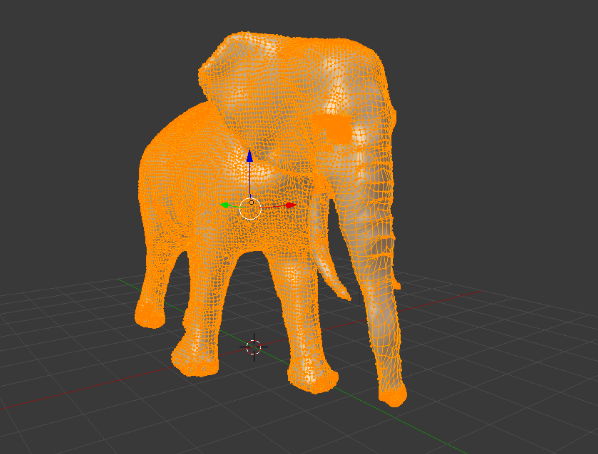
\includegraphics[width=\linewidth]{elefant_viele_polygone.png}
  \caption{Polygonnetz vor Bearbeitung}\label{fig:elefant_viele_polygone}
\endminipage\hfill
\minipage{0.48\textwidth}
  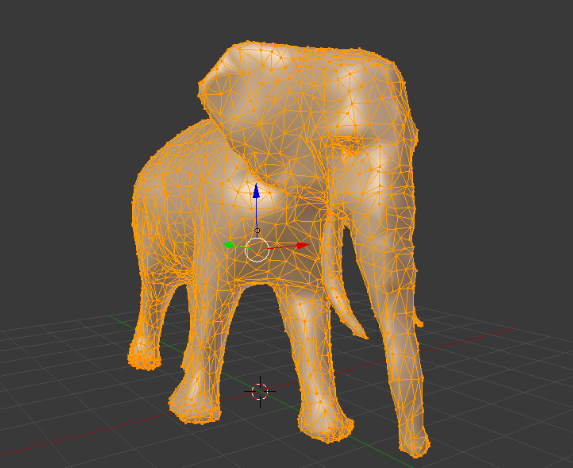
\includegraphics[width=\linewidth]{elefant_wenig_polygone.png}
  \caption{Polygonnetz nach Bearbeitung}\label{fig:elefant_wenig_polygone}
\endminipage\hfill
\end{figure}

Aus Grafik \ref{fig:elefant_wenig_polygone} geht hervor, dass sich die Gestalt des 3D Objektes trotz verringerter Polygonzahl kaum verändert und der Prozess der Polygonreduktion somit zu einem nicht merklichen Genauigkeitsverlust führt.
\subsection{Einbindung der 3D Objekte in Unity}\label{einbindung_3D_objekte}
Der Zugriff auf die ausgewählten 3D Objekte innerhalb des Unity-Entwicklungsoberfläche, sowie der Applikation wird ermöglicht, indem die Objekte im Projektpfad als Ressourcen abgelegt werden, welche beim Bauen der Applikation auf das Endgerät mit übertragen werden. 

Wie in Abschnitt, \ref{projektziel} beschrieben, soll ein 3D Objekt nur bei der Erkennung des ihm zugeordneten Landes angezeigt werden.
Um dies zu realisieren, werden die 3D Objekte in der Entwicklungsoberfläche als Kind-Objekte der in Abschnitt \ref{integration_image_targets} beschriebenen Image-Targets angelegt.
Das Verhalten dieser Vuforia-Elemente wird durch das \textquote{DefaultTrackableEvent-Handler}-Skript bestimmt, welches den Elementen standardmäßig beigefügt ist. 
Bei der Feuerung des \textquote{OnTrackableFound}-Events, das heißt der Erkennung eines Image-Targets, werden die diesem untergeordneten, renderbaren Kindelemente mithilfe der von Unity bereitgestellten \textquote{Renderer}-Klasse automatisch gerendert.

Das beschriebene \textquote{DefaultTrackable-EventHandler}-Skript kann nach Belieben bearbeitet werden, um ein besonderes, durch den Benutzer gewünschtes Verhalten hervorzurufen.
In unserem Fall wurde das \textquote{OnTrackable-Found}-Event so überschrieben, dass zusätzlich zu dem 3D Objekt noch zwei Buttons angezeigt werden, mit welchen der User interagieren kann.

\section{Verwaltung der Daten}
\subsection{Datenbankentwurf}\label{datenbankentwurf}
\subsection{Zugriff auf Datenbankinhalte}\label{zugriff_datenbank}

\section{Realisierung der Anwendung in Unity}
Den generellen Aufbau einer Unity-Anwendung haben wir bereits im Kapitel \ref{aufbau_unity_app} erläutert.
Wie unsere Anwendung nun aufgegliedert ist wird im nachfolgenden Teil behandelt.

Insgesamt besteht die Applikation aus 8 Szenen. Angefangen mit der Menüszene, von der aus man entweder in die Onboarding-Szene für das Tutorial, den Spiel- oder den Informationsteil gelangt. 
Der Spiel- und der Informationsteil setzen sich wiederum aus eigenen Szenen zusammensetzen, zu welchen in den nächsten beiden Abschnitten mehr Informationen folgen. 

\subsection{Informationsbereich}
%aus welchen Szenen besteht der Teil
Der Informationsteil besteht aus vier Einzelszenen. 
In den ersten beiden wählt der Nutzer einen Kontinent und dann ein Land über das er etwas erfahren möchte.
Daraufhin folgt eine Zwischenszene, welche als Vorschau für das gewählte Land dient und danach startet die eigentliche Informationsszene. 

Um den ganzen Bereich Dynamisch zu halten, befinden sich in den Szenen nur Dummyobjekte, welche noch nicht mit Texten befüllt sind. Das heißt, dass beispielsweise die Kontinentauswahl vorerst nur leere Buttons und die Informationsszene leere Informationsfelder enthält.
Durch die in Abschnitt \ref{zugriff_datenbank} beschriebene Datenbankschnittstelle, kommt nun beim Laden dieser Szenen der Inhalt hinzu. 
Die leeren Auswahlbuttons in der Kontinent- und der Länderszene werden mit Texten und Farben befüllt. Und die leeren Informationsfelder werden mit hilfreichen Fakten beschrieben.

Anhand der Informationsszene kann man dies sehr gut veranschaulichen. 
Beim tippen auf eines der wählbaren Länder wird das Behaviour-Script der aktuellen Szene aufgerufen, in dem sich ein onClick-Event befindet. 
In diesem wird der Inhalt des angeklickten Objekts ausgelesen und zwischengespeichert. Nun kann er als Parameter an die Datenbankfunktion weitergereicht werden, welche für das Laden der Informationen eines Landes zuständig ist. 
Die daraus resultierenden Daten stehen nun in der darauffolgenden Szene in Form einer Liste zur Verfügung.
Die darauffolgende Szene ist nun die Informationsszene. Deren leere Informationsfelder bestehen aus mehreren GameObjects.
Aus dem Hintergrundbild welches als Container der Informationen dient und aus dem eigentliche Textobjekt.
Beim Laden dieser Szene wird jedes mal eine Funktion ausgeführt, welche die vorher erlangten Daten verarbeitet.
Es wird mithilfe einer Schleife über die zwischengespeicherten Informationstexte iteriert, und für jeden Textblock in der Szene wird das jeweilige Textattribut ersetzt.

\subsection{Quizbereich}
Ein sehr ähnliches Grundprinzip wurde bei der Umsetzung der Quizszene verfolgt.
Wie auf Abbildung \ref{fig:quizscene} zu sehen, wurde ebenfalls die Benutzeroberfläche mit GameObjects vormodelliert und dessen Textinhalte bestehen noch aus Platzhalterwerten.

\begin{figure} [h]
\centering
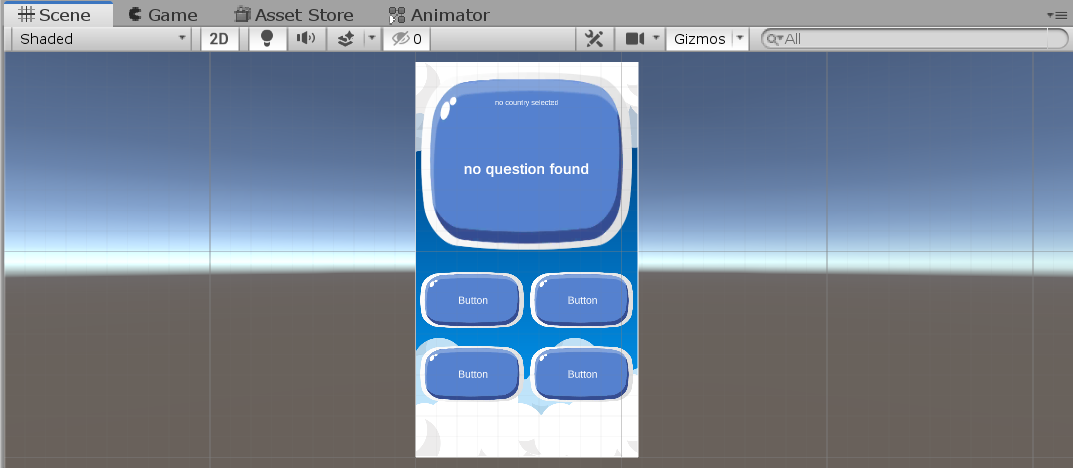
\includegraphics[width=14cm]{quiz_scene.PNG}
\caption{Initialer Status der Quizszene}
\label{fig:quizscene}
\end{figure}

Beim initialen Laden der Szene benötigen wir zu aller erst die Frage- und Antwortdaten des jeweiligen Landes aus der Datenbank.
Dafür werden wieder Methoden aus der Datenbankschnittstelle, mit dem Übergabeparameter des angeklickten Landes aufgerufen. 
Zuerst laden wir alle Fragen zu dem Land und daraufhin alle Antwortmöglichkeiten zu jeder Frage. 
Die Antwortmöglichkeiten werden an das generierte Frageobjekt angehängt und so entsteht eine Liste aus vollständig zusammengesetzten Frageentitäten.
Diese Liste wird nun innerhalb der Quizszene abgespeichert und kann jetzt wie im vorher beschriebenen Informationsteil zum Befüllen der Szene genutzt werden.

Hierfür benötigen wir ein C\#-Script, welches das Verhalten der gesamten Quizszene kontrolliert.
Dieses liegt als eigenes GameObject innerhalb der Szene und hält Referenzen auf die in der Szene liegenden GameObjects.
Wir referenzieren alle UI-Elemente die wir zum Laden des Quiz benötigen.
Dies sind der Fragetext, der Text des aktuellen Landes und die vier Buttons der Auswahlmöglichkeiten.

Nun benötigen wir Logik, die über die vorhandenen Fragen iteriert und für jedes Frageobjekt die UI-Texte neu befüllt. Das geschieht innerhalb einer Methode im Script, welche für jede Frage erneut aufgerufen wird. 
Mittels einer Zählervariable weiß sie, welche Frage gerade aktiv ist und befüllt die Szenenoberfläche mit deren Daten.
Hierfür sind die referenzierten GameObjects notwendig, da über sie die Platzhaltertexte überschrieben werden können. 

Damit sich die Reihenfolge der Antwortmöglichkeiten nicht bei jedem Quizdurchlauf wiederholt, mischen wir sie vorher durch. 
Nun müssen wir den Buttons noch onClick-Funktionalität geben. 
Ist eine Antwortmöglichkeit mit dem flag für \textquote{isCorrectAnswer} versehen, zählt ihr onClickListener einen Zähler hoch und ruft anschließend die Initialisierung der nächsten Frage auf. 
Falls nicht bleibt der Zähler gleich und es wird ebenfalls die nächste Frage geladen.